\documentclass[12pt]{article}
\title{EE445M Lab 4}
\author{Hershal Bhave (hb6279) and Eric Crosson (esc625)}
\date{Friday April 03, 2015}

\usepackage[in]{fullpage}
\usepackage{listings}
\usepackage{cleveref}
\usepackage[nosolutionfiles]{answers}
\usepackage{graphicx}
\usepackage{xcolor}
\usepackage{color}
\usepackage{enumerate}
\usepackage{pdfpages}

\newenvironment{Ex}{\textbf{Problem}\vspace{.75em}\\}{}
\Newassociation{solution}{Soln}{Answers}
\pagebreak[3]
\newcommand{\Opentesthook}[2]{\Writetofile{#1}{\protect\section{#1: #2}}}
\renewcommand{\Solnlabel}[1]{\textbf{Solution}\quad}
\newcommand{\todo}{{\LARGE \emph{\color{red}TODO}}}

\newcommand{\dd}[1]{\:\mathrm{d}{#1}}
\newcommand{\ddt}[1]{\frac{\dd{}}{\dd{#1}}}
\newcommand{\dddt}[1]{\frac{\dd{}^2}{\dd{#1}^2}}

\definecolor{mygreen}{rgb}{0,0.6,0}
% \definecolor{mygreen}{rgb}{0.13,0.55,0.13}
\definecolor{mygray}{rgb}{0.5,0.5,0.5}
\definecolor{mymauve}{rgb}{0.58,0,0.82}

\lstset{
  backgroundcolor=\color{white},
  basicstyle=\scriptsize\ttfamily,
  breakatwhitespace=false,
  breaklines=true,
  captionpos=b,
  commentstyle=\color{mygreen},
  deletekeywords={...},
  escapeinside={\%*}{*)},
  extendedchars=true,
  frame=single,
  keywordstyle=\color{blue},
  % language=Octave,
  % numbers=left,
  % numbersep=5pt,
  % numberstyle=\tiny\color{mygray},
  rulecolor=\color{black},
  showspaces=false,
  showstringspaces=false,
  showtabs=false,
  % stepnumber=2,
  stringstyle=\color{mymauve},
  tabsize=2,
  title=\lstname,
  columns=fullflexible,
}

\begin{document}
\maketitle

\section{Objectives}
\begin{itemize}
  \item Interface a microphone and record sounds
  \item Design and implement an analog HPF, LPF and digital FIR filters
  \item Build a spectrum analyzer
  \item Write a real-time application that displays in both the time domain and the frequency domain
\end{itemize}

\section{Hardware Design}
Attached is a TI Webench Design Report of the analog low pass filter
used in this lab.
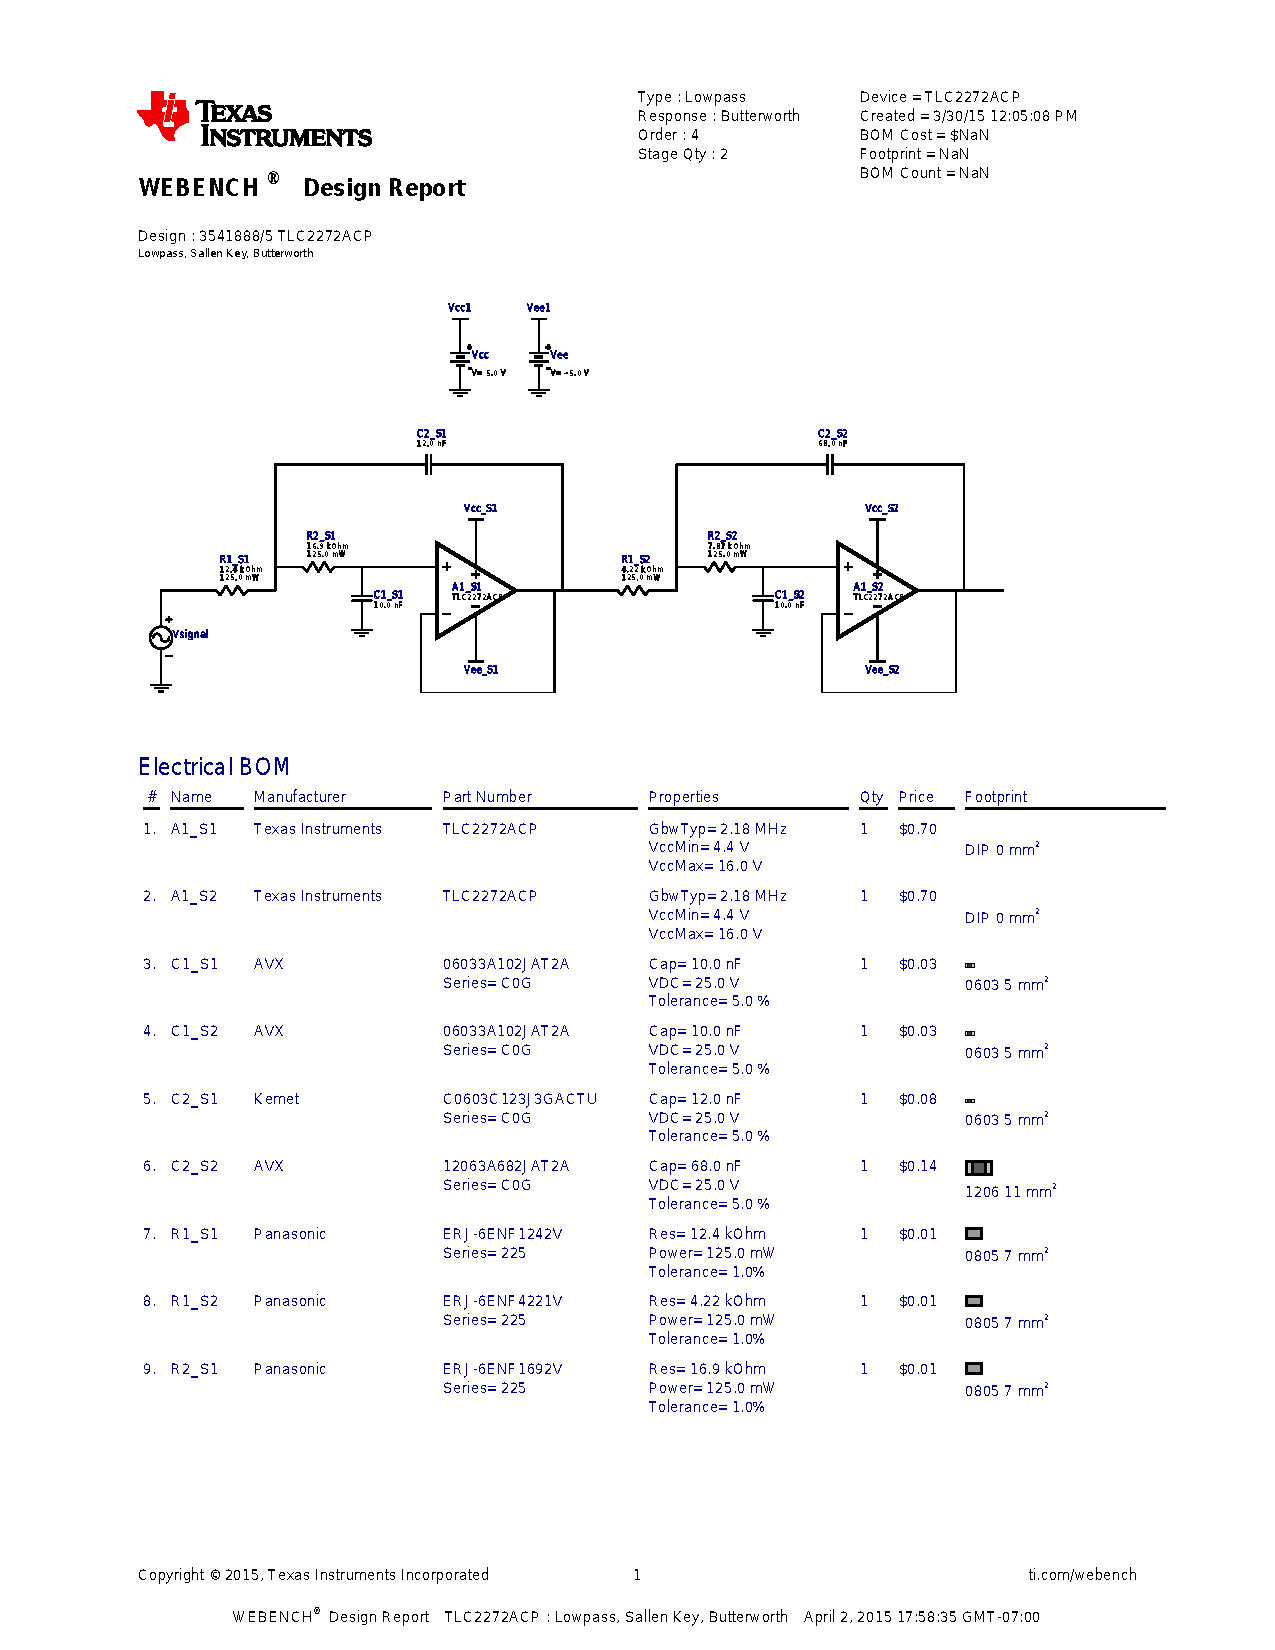
\includepdf[pages={1}]{./img/webench_analog_filter.pdf}

\section{Software Design}
Reference \cref{lst:lab4}. No extra magic is happening here - we have
distinct functions to handle the data manipulation (filtering, fft)
and discrete modes of operation. Semaphores guard shared resources and
timers dictate periodic tasks. Users may switch between
modes by entering commands through the shell via UART.

To facilitate debugging, we found it convenient to monitor operations
in the absence of periodic timer interrupts. Since SysTick is
responsible for the task switching, the only functionality periodic
timers were giving us related to ADC sampling at a specific rate. Each
trigger for ADC sampling started a lengthy data acquisition
process. To mitigate the need to work around these events while
debugging we introduce an adc simulator. The method
\verb|simulate_adc| iterates over a sine wave in memory and feeds the
sequential values into the FIFO that normally takes information from
the ADC. As such, normal program execution continues with
``simulated'' signals from a nonexistent signal generator.

Testing of each component (plot graphics, data acquisition, filter
accuracy, FFT) was by visual examination of output through the
LCD.

\section{Measurement Data}
\begin{enumerate}[a)]
  \item Dynamic circuit performance
  \item Digital scope data
  \item Spectrum analyzer data
  \item FIR filter test data
\end{enumerate}

\section{Analysis and Discussion}
\begin{enumerate}[1)]
  \item todo
\end{enumerate}

\section{Code}
\lstinputlisting[language=C,label=lst:lab4,caption=\texttt{lab4.c}]{@doc-staging-area@/lab4.c}

\end{document}
